

\chapter{Spatial discretization}


Consider the 1D advection equation

\begin{equation}
\frac{\partial f}{\partial t} = -u\frac{\partial f}{\partial x}
\end{equation}

and let us discretize it in time and space. There are different ways
we can approximate the spatial derivative

\beqn
\frac{\partial f}{\partial x} &\approx& \frac{f_i -
  f_{i-1}}{\Delta x} \quad \mathrm{FTBS \ forward \ time \ back \ space}\\
\frac{\partial f}{\partial x} &\approx& \frac{f_{i+1} -  f_i}{\Delta  x} \quad \mathrm{FTFS \ forward \ time \ foward \ space}\\
\frac{\partial f}{\partial x} &\approx& \frac{f_{i+1} -  f_{i-1}}{2\Delta x}\quad \mathrm{FTBS \ forward \ time \ center \ space}\\
\frac{\partial f}{\partial x} &\approx& \frac{f_{i+1/2} - f_{i-1/2}}{\Delta x}
\eeqn


Let us pick the centered 

\begin{equation}
\frac{f^{(n+1)}_i - f^{(n)}_i}{\Delta t } = - u \left( \frac{f^{(n)}_{i+1} - f^{(n)}_{i-1}}{2\Delta x}\right)
\end{equation}


We isolate the quantity we want to find, $f_i$ in the future

\begin{equation}
f^{(n+1)}_i  = f^{(n)}_i - \frac{u\Delta t}{2\Delta x} \left( f^{(n)}_{i+1} - f^{(n)}_{i-1}\right)
\end{equation}

We define the {\bf Courant number}, which is a dimensionless quantity
that, as we see later, determines the {\it stability} of the different schemes

\begin{equation}
\boxed{
C \equiv \frac{u\Delta t}{\Delta x}
}
\end{equation}

In terms of the Courant number, the recurrence relation is 
\begin{equation}
f^{(n+1)}_i  = f^{(n)}_i - \frac{C}{2} \left( f^{(n)}_{i+1} - f^{(n)}_{i-1}\right)
\end{equation}


\subsection{Stencil Diagrams}

The field $f_i^{(n+1)}$ at grid point $i$ and time step $n + 1$
depends on values at the old time step $n$. This is sketched in a
so-called {\it stencil diagram}. 

\begin{figure}
  \begin{center}
    \resizebox{\textwidth}{!}{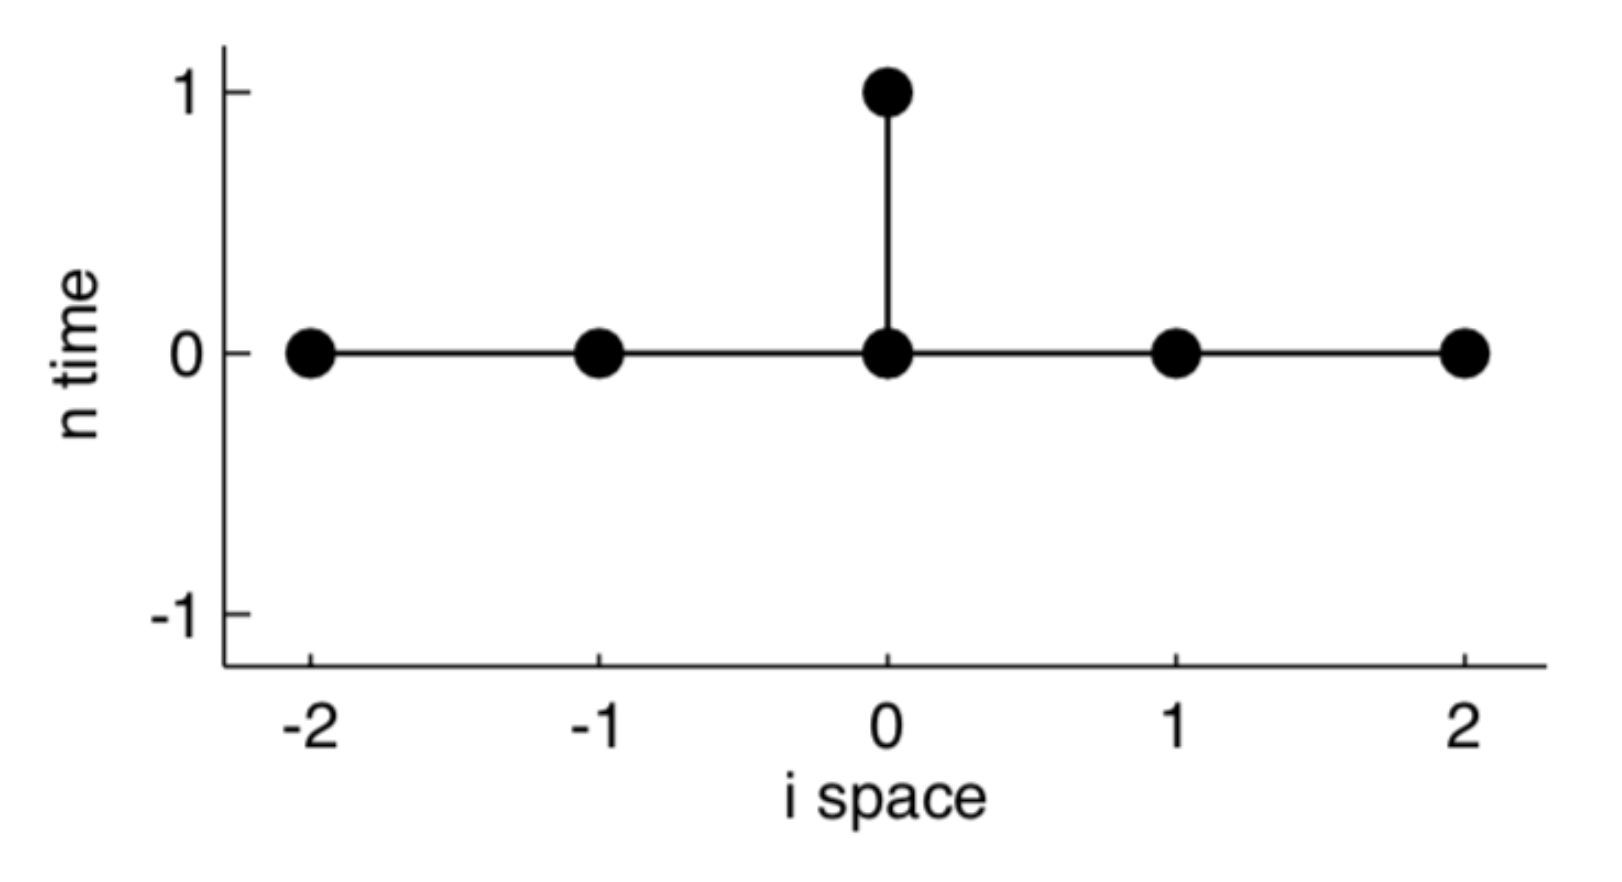
\includegraphics{./figs/stencil1.png}}
  \end{center}
  \caption[]{Stencil diagram}
  \label{fig:stencil1}
\end{figure}

\subsection{``Naive'' scheme}

%The ``naive'' scheme averages the adjacent grid points 

%\begin{equation}
%f_{i+1/2} = \frac{v}{2}\left(\rho_{i+1} + \rho_i\right)
%\end{equation}

%Leading to 

Consider the equation we obtained 

\begin{equation}
f^{(n+1)}_i  = f^{(n)}_i - \frac{C}{2}\left(f_{i+1} - f_{i-1}\right)
\end{equation}


\begin{figure}
  \begin{center}
    \resizebox{\textwidth}{!}{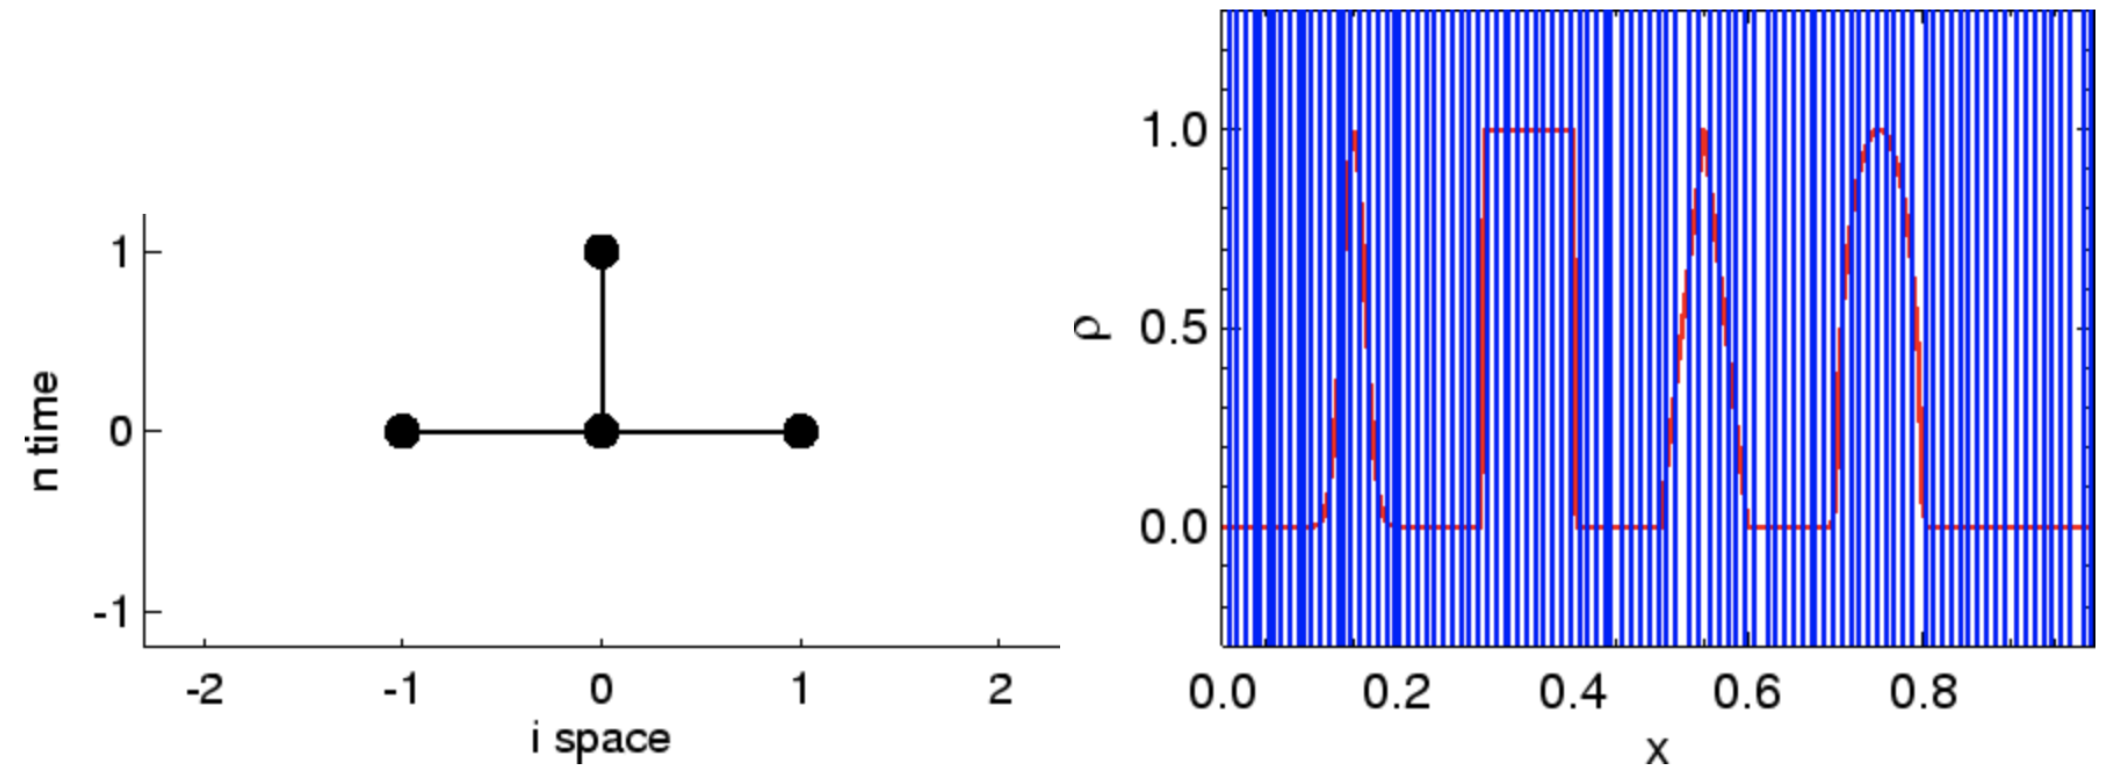
\includegraphics{./figs/naive.png}}
  \end{center}
  \caption[]{Centered difference ``naive'' scheme}
  \label{fig:naive-adv}
\end{figure}


The solution is shown in \fig{fig:naive-adv}. The oscillations are
seen to grow exponentially \figp{fig:naive-adv}. After some time the
numerical result does not have the faintest resemblance to true
solution. We will call this scheme ``naive''. 

\subsection{Von-Neumann stability analysis}

Why does the naive scheme fail so drastically? Let us look at a Fourier mode of the function

\begin{equation}
f(x,t) = A(t) e^{-ikx}
\end{equation}


The naive scheme turns into

\begin{equation}
A(t+\Delta t)e^{-ikx} = A(t)e^{-ikx} - \frac{C}{2}A(t)\left[e^{-ik(x+\Delta x)} - e^{-ik(x-\Delta x)}\right]
\end{equation}

multiplying by $e^{ikx}$


\begin{equation}
A(t+\Delta t) = A(t) \left[ 1 - \frac{C}{2}\left(e^{-ik\Delta x} -  e^{ik\Delta x}\right)\right]
\end{equation}

the term in parentheses in the RHS is the sine function

\classcomm{If class doesn't recognize it as the sin function, show quickly using Euler formula
  \beqn
  e^{ix}  &=& \cos x + i \sin x\\
  e^{-ix}  &=& \cos x - i \sin x\\
  \eeqn
  which leads to
  \beqn
  \cos x &=& \frac{e^{ix} + e^{-ix}}{2}\\
  \sin x &=& \frac{e^{ix} - e^{-ix}}{2i}\\
  \eeqn
}
  

\begin{equation}
A(t+\Delta t) = A(t)\left[1 + i C \sin \left(k\Delta x\right)\right]
\end{equation}

multiplying by the complex conjugate we find the amplitude

\begin{equation}
A^2(t+\Delta t) = A^2(t)\left[1 + C^2 \sin^2\left(k\Delta x\right)\right]
\end{equation}

We see that the amplitude of any wave, irrespective of $k$, will always increase, independently of the Courant number. The scheme is unconditionally unstable. 

\subsection{Back space (upwinding)}

\begin{figure}
  \begin{center}
    \resizebox{\textwidth}{!}{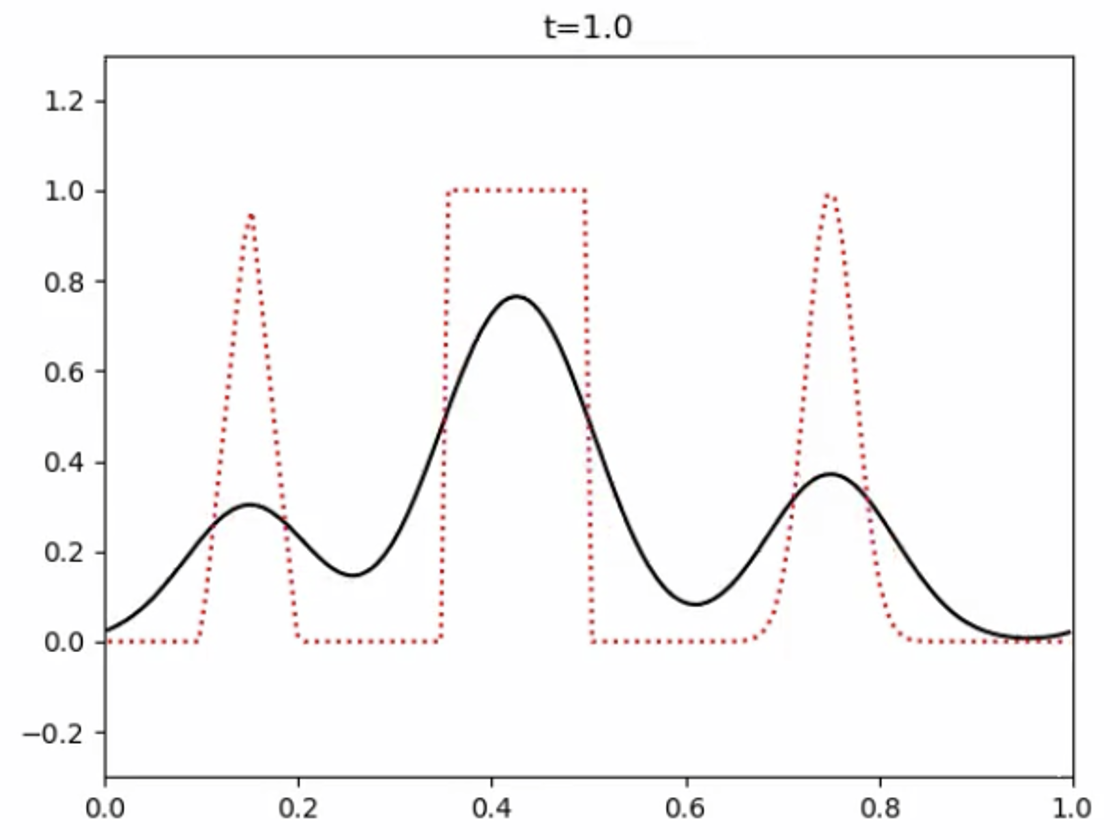
\includegraphics{./figs/donor.png}}
  \end{center}
  \caption[]{Donor cell}
  \label{fig:donor}
\end{figure}

The back space scheme uses the point upwind
(back space) for the derivative. The scheme results in 

\begin{equation}
f^{(n+1)}_i  = (1-C) f^{(n)}_i + Cf^{(n)}_{i-1}
\end{equation}

The stencil is sketched in \fig{fig:donor}. It depends on the point and the point immediately upwind. The Courant number is the weight given to the upwind point. 

The result is smooth but smeared out severely. Let us look at the von Neumann stability analysis upwind scheme. Using again a single Fourier mode 


\begin{equation}
f(x,t) = A(t) e^{-ikx}
\end{equation}

The upwind scheme turns into

\begin{equation}
A(t+\Delta t)e^{-ikx}  = (1-C) A(t)e^{-ikx} + CA(t)e^{-ik(x-\Delta x)}
\end{equation}

multiplying by $e^{ikx}$

\begin{equation}
A(t+\Delta t)  = A(t) \left(1 - C  +C e^{ik\Delta x}\right)
\end{equation}


expaning the exponential 

\begin{equation}
A(t+\Delta t)  = A(t) \left(1 - C + C\cos k\Delta x + C i\sin k\Delta x\right)
\end{equation}

Replacing $B = 1 - C + C\cos k\Delta x$ and $D = C\sin k\Delta x$

\begin{equation}
A(t+\Delta t)  = A(t) \left(B + iD\right)
\end{equation}

multiplying by the complex conjugate 

\begin{equation}
A^2(t+\Delta t)  = A^2(t) \left(B^2  + D^2\right)
\end{equation}

where the amplification factor is 

\begin{eqnarray}
B^2+D^2 &=& \left(1 - C + C\cos k\Delta x\right)^2 + C^2\sin^2 k\Delta x\\
&=&(1-C)^2 + 2(1-C)C\cos k\Delta x 
\end{eqnarray}


The maximum and minimum values of $\cos k\Delta x$ are 1 and -1, so the amplification is bound between 

\begin{equation}
(1-C)^2 - 2(C-C^2) \leq B^2+D^2 \leq (1-C)^2 + 2(C-C^2) 
\end{equation}

For the maximum amplification to be below 1 we require 

\begin{equation}
0 \leq 1 - C^2 \leq 1 
\end{equation}

which is true for 

\begin{equation}
\boxed{
C \leq 1
}
\end{equation}

This is the {\it condition of stability} of the upwind scheme.

Upwinding seems promising to achieve stability. However, the accuracy
of the scheme has to be improved.

Note on the nature of the ``smoothing'' of the solution. Even though
the advection equation does not have any diffusion in it, the
numerical algorithm to solve this advection equation intrinsically has
some diffusion. In fact, there exists no numerical method without
numerical diffusion. Some algorithms have more of it, some have less,
and there exist method to constrain the smearing-out of
discontinuities. But in principle numerical diffusion is
unavoidable.

One way of seeing this is by doing the following exercise. Consider the upwind scheme. It
uses the derivative $i- 1/2$ for the update of the state at $i$. So let us write the derivative at $i- 1/2$ as:

\beq
\frac{f_i-f_{i-1}}{\Delta x} = \frac{q_{i+1}-q_{i-1}}{2\Delta x} -
\Delta x \frac{f_{i+1}-2f_i+f_{i-1}}{2\Delta x^2}
\eeq

The left-hand-side is the upstream difference, the first term on the
right-hand-side is the centered difference and the second term on the
right-hand-side can be recognized as a diffusion term with diffusion constant

\beq
D=\frac{u\Delta x}{2}
\eeq

This shows that the upstream difference scheme can be regarded to be the same as the centered
difference scheme supplemented with a diffusion term. The pure centered difference scheme
is unstable, but once a bit of diffusion is added, the algorithm stabilizes. The drawback is,
however, that the diffusion smears any features out. If one would define the centered difference
formulation of the x-derivative as the ``true'' derivative (which is of course merely a definition),
then the numerical diffusion of the upstream differencing scheme is
quantified by D as given in the equation above. 

In practice it is not possible to perfectly define the diffusivity of an algorithm since the
centered difference formulation of the derivative is also merely an approximation of the true
derivative. But it is nevertheless a useful way of looking at the concept of numerical diffusion.
In principle one could say that it is as if we are solving

\beq
\frac{\partial f}{\partial t} = - u \frac{\partial f}{\partial x} +\frac{u\Delta x}{2}\frac{\partial^2 f}{\partial^2 x}
\eeq

Clearly, for $\Delta x \rightarrow 0$ the diffusion vanishes. This is obviously a necessary condition, otherwise
we would be modeling the true diffusion equation, which is not what we want. The diffusion
that we see here is merely a by-product of the numerical algorithm we
used. Note that sometimes (as we shall see below) it is useful to add
some viscosity on purpose to an algorithm. This is called artificial
viscosity. One could therefore say that the upstream differencing is equal to centered differencing plus artificial viscosity.

\section{Taylor series}

Taylor series are  expansions of a function $f(x)$ for some 
finite distance $\Delta x$ to $f(x+\Delta x)$

\beq
f(x\pm \Delta x) = f(x) \pm \Delta x f^\prime(x) + \frac{\Delta
  x^2}{2} f^{\prime\prime}(x) \pm \frac{\Delta x^3}{3!}
f^{\prime\prime\prime}(x) + \frac{\Delta
  x^4}{4!} f^{\prime\prime \prime\prime}(x) \pm ...
\eeq

What happens, if we use this expression for the forward derivative

\beq
\frac{\partial f}{\partial x} \approx \frac{f(x+\Delta x) - f(x)}{\Delta x}
\eeq

which leads to

\beqn
\frac{f(x+\Delta x) - f(x)}{\Delta x} &=& \frac{1}{\Delta x} \left[ \Delta x f^\prime(x) + \frac{\Delta
  x^2}{2} f^{\prime\prime}(x) + \frac{\Delta x^3}{3!}
f^{\prime\prime\prime}(x)\right]\\
&=&f^\prime(x) + \mathcal{O}\left(\Delta x\right)
\eeqn

The error of the first derivative using the forward 
formulation is of order $\Delta x$. Is this the case for other formulations of the derivative?
Let’s check.

With the centered formulation we get:

\beqn
\frac{f(x+\Delta x/2) - f(x-\Delta x/2)}{\Delta x} &=&\frac{1}{\Delta
  x} \left[ \Delta x f^\prime(x) + \frac{\Delta
    x^2}{3!}f^{\prime\prime\prime}(x)+...\right]\\
&=&f^\prime(x) + \mathcal{O}(\Delta x^2)
\eeqn

The error of the first derivative using the centered 
approximation is of order $\Delta x^2$. This is an important result: it does matter which formulation
we use. The centered scheme is more accurate. Yet, we just saw that
the more accurate one is unstable, whereas the less accurate one is
stable. {\it Accuracy does not guarantee stability.}

\section{High-order finite-difference derivatives}

The first derivative, to 2nd order accuracy is 

\begin{equation}
f_i^\prime = \frac{-f_{i-1} + f_{i+1}}{2\Delta x} + \mathcal{O}(\Delta x^2)
\end{equation}

to 4th order accuracy, it is 

\begin{equation}
f_i^\prime = \frac{f_{i-2} -8f_{i-1} +8f_{i+1} - f_{i+2}}{12\Delta x} + \mathcal{O}(\Delta x^4)
\end{equation}

to 6th order accuracy, it is 

\begin{equation}
f_i^\prime = \frac{-f_{i-3} + 9f_{i-2} -45f_{i-1} +45f_{i+1} -9f_{i+2} + f_{i+3}}{60\Delta x} + \mathcal{O}(\Delta x^6)
\end{equation}

The table shown in \fig{fig:tablecoefficients} shows the coefficients (weights) given to each point on computing a derivative to desired accuracy. We will draw from this table to compute first and second derivatives, mostly. But how are these coefficients determined?  

\begin{figure}
  \begin{center}
    \resizebox{\textwidth}{!}{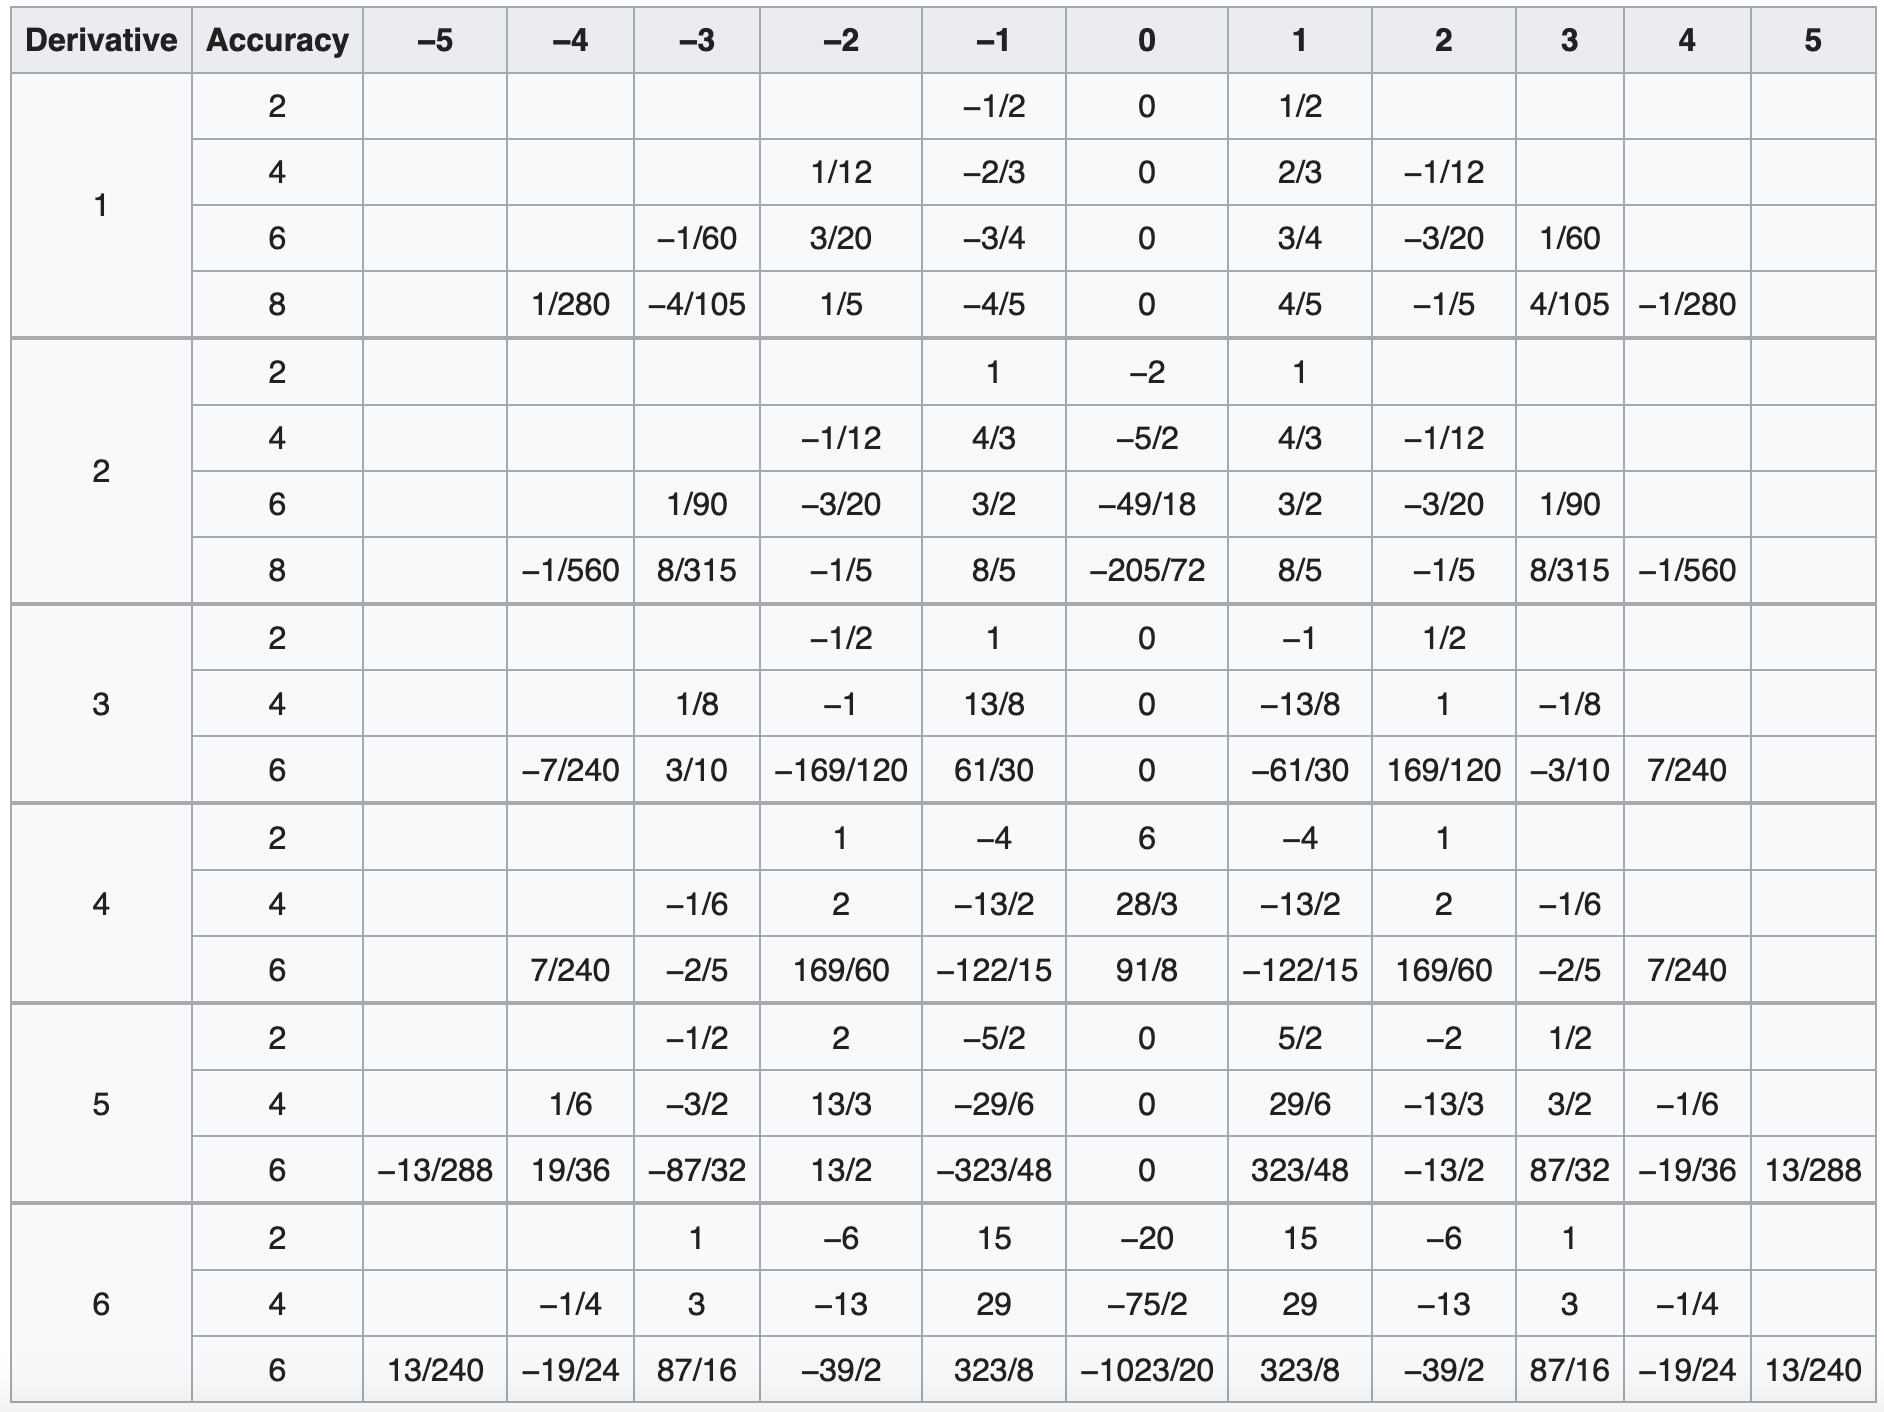
\includegraphics{./figs/tablecoefficients.png}}
  \end{center}
  \caption[]{}
  \label{fig:tablecoefficients}
\end{figure}

These coefficients come from Taylor expansion. Suppose that we want to compute df/dx to 2nd order. Using a 3-point stencil, we have 

\begin{equation}
\frac{df}{dx} = \frac{1}{h}\left[Af(x-h) + Bf(x) + Cf(x+h)\right]
\end{equation}

where $h=\Delta x$. According to the table in \fig{fig:tablecoefficients}, we expect to find $A=-1/2$, $B=0$ and $C=1/2$. Let us prove this.

If we Taylor expand around $x$, 

\begin{eqnarray}
Af(x-h) &=& Af(x) + Af^\prime(x)(-h) + Af^{\prime\prime}(x)\frac{h^2}{2}  \\
Bf(x)   &=& Bf(x)   \\
Cf(x+h) &=& Cf(x) + Cf^\prime(x)(h) + Cf^{\prime\prime}(x)\frac{h^2}{2} 
\end{eqnarray}

Summing them all 

\begin{equation}
h\frac{df}{dx} = f(x)(A+B+C) + f^\prime(x)(A-C)h + f^{\prime\prime}(x)\frac{h^2}{2}(A+C) 
\end{equation}

Since only the first derivative should survive in the RHS, this leads to the conditions 

\begin{eqnarray}
A+B+C&=&0\\
A-C &=& 1\\
A+C &=& 0 
\end{eqnarray}

Leading to $A=-1/2$, $C=1/2$, $B=0$, as expected.


Another example, find the fourth derivative $d^4f/dx^4$, with a 5-point stencil 


\begin{equation}
h^4\frac{d^4f}{dx^4} = Af(x-2h) + Bf(x-h) + Cf(x) + Df(x+h) + Ef(x+2h)
\end{equation}

Expanding the terms in Taylor to fourth order 

\begin{eqnarray}
Af(x-2h) &=& Af(x) + Af^\prime(x)(-2h) + Af^{\prime\prime}(x)\frac{(2h)^2}{2}  + Af^{\prime\prime\prime}(x)\frac{(-2h)^3}{6}+ Af^{\prime\prime\prime\prime}(x)\frac{(2h)^4}{24}\nonumber\\
Bf(x-h) &=& Bf(x) + Bf^\prime(x)(-h) + Bf^{\prime\prime}(x)\frac{h^2}{2}  + Bf^{\prime\prime\prime}(x)\frac{(-h)^3}{6}+ Bf^{\prime\prime\prime\prime}(x)\frac{h^4}{24}\nonumber\\
Cf(x) &=& Cf(x) \\
Df(x+h) &=& Df(x) + Df^\prime(x)(h) + Df^{\prime\prime}(x)\frac{h^2}{2}  + Df^{\prime\prime\prime}(x)\frac{h^3}{6}+ Df^{\prime\prime\prime\prime}(x)\frac{h^4}{24}\nonumber\\
Ef(x+2h) &=& Ef(x) + Ef^\prime(x)(2h) + Ef^{\prime\prime}(x)\frac{(2h)^2}{2}  + Ef^{\prime\prime\prime}(x)\frac{(2h)^3}{6}+ Ef^{\prime\prime\prime\prime}(x)\frac{(2h)^4}{24}\nonumber
\end{eqnarray}

And grouping together the terms with same order in the derivative

\begin{eqnarray}
f(x)[A+B+C+D+E] &=& 0\\
f^\prime(x)h[-2A-B+D+2E] &=& 0\\
f^{\prime\prime}(x)\frac{h^2}{2}[(-2)^2+B +D+2^2E] &=& 0\\
f^{\prime\prime\prime}(x)\frac{h^3}{3!}[(-2)^3A-B +D+2^3E]&=&0\\
f^{\prime\prime\prime\prime}(x)\frac{h^4}{4!}[(-2)^4A+B +D+2^4E]&=&f^{\prime\prime\prime\prime}(x)h^4
\end{eqnarray}

The system  is 

\begin{eqnarray}
A+B+C+D+E &=& 0 \\
-2A-B+D+2E &=& 0 \\
4A+B +D+4E &=& 0 \\
-8A-B +D+8E &=&0 \\
16A+B +D+16E &=&4!
\end{eqnarray}


In matrix form this equation is 

\begin{equation}
\left[
\begin{array}{ccccc}
1&1&1&1&1\\
-2&-1&0&1&2\\
4&1&0&1&4\\
-8&-1&0&1&8\\
16&1&0&1&16
\end{array}\right]
\left[
\begin{array}{c}
A\\
B\\
C\\
D\\
E
\end{array}\right]=4!\left[
\begin{array}{c}
0\\
0\\
0\\
0\\
1
\end{array}\right]
\end{equation}

This yields $(A,B,C,D,E)=(1,-4,6,-4,1)$ as shown below. 

\begin{mintedbox}{python}
a=np.zeros([5,5]) 

s=[-2,-1,0,1,2]

for i in range(5):
    for j in range(5):
        a[i,j] = s[j]**(i) 

a_inv = np.linalg.inv(a)
rhs=24 * np.transpose([0,0,0,0,1])
coefficients=np.matmul(a_inv,rhs) 
print(coefficients)
\end{mintedbox} 

[ 1. -4.  6. -4.  1.]


In general, this recurrence relationship is 

\begin{equation}
(-2)^n A + (-1)^nB + 0^n C + 1^nD + 2^nE = 4! \ \delta(n-4)
\end{equation}

We can distill from this the general formula. The bases are the set of stencil positions, $s=(-2,-1,0,1,2)$. The coefficients $c$ (in this case, $A$ to $E$) are set by 

\begin{equation}
\boxed{
\sum_{i=0}^{N-1} s_i^n c_i = d! \ \delta(n-d) \quad \mbox{for $0 < n < N-1$} 
}
\end{equation}


where $N$ is the size of the stencil, and $d$ the order of the derivative. 

Let us calculate with this formula the second derivative to 4th order accuracy, with a 5-point stencil.

\begin{equation}
\left[
\begin{array}{ccccc}
1&1&1&1&1\\
-2&-1&0&1&2\\
4&1&0&1&4\\
-8&-1&0&1&8\\
16&1&0&1&16
\end{array}\right]
\left[
\begin{array}{c}
a_1\\
a_2\\
a_3\\
a_4\\
a_5
\end{array}\right]=2\left[
\begin{array}{c}
0\\
0\\
1\\
0\\
0
\end{array}\right]
\end{equation}

\begin{mintedbox}{python}
rhs=2 * np.transpose([0,0,1,0,0])
coefficients=np.matmul(a_inv,rhs) 
print(coefficients)
\end{mintedbox} 

[-0.08333333  1.33333333 -2.5         1.33333333 -0.08333333]

In rational numbers, these are -1/12, 4/3, 5/2, 4/3, -1/12, exactly as
stated in the table in \fig{fig:tablecoefficients}.

\section{Effective wavenumber}

Given a Fourier signal $\cos(kx)$, the spatial derivative is

\beq
\frac{d\left(\cos kx \right)}{dx} = -k\sin kx
\eeq

this means that we can equate

\beq
k = -\frac{1}{\sin kx}\frac{d\left(\cos kx \right)}{dx} 
\eeq

numerically, the derivative is not perfect, so measuring the numerical
result of the RHS (the throughput) is a measure of the accuracy of the
numerical scheme:

\beq
k_{\rm eff} = -\frac{1}{\sin kx}\left.\frac{d\left(\cos kx
  \right)}{dx}\right\vert_{\rm numerical} 
\eeq

Or, to avoid dividing by zero

\begin{itemize}

\item Define a vector $\v{A} = (0, sin kx, cos kx)$.
\item Note that $\v{B} = \curl{\v{A}}= k\v{A}$.
\item Evaluate numerically $\v{A}\cdot \v{B}$
\item Since $|\v{A}|=1$ we find immediately the effective wavenumber
  as $k_{\rm eff} = \langle \v{A}\cdot\v{B}\rangle$.

\end{itemize}
  
Similarly for the second derivative 

\beq
k^2 = \frac{1}{\cos kx}\frac{d^2\left(\cos kx \right)}{dx^2} 
\eeq

and the effective: 

$k^2_{\rm eff} = \langle \v{A}\cdot\v{J}\rangle$, where $\v{J} =
-\Laplace{\v{A}}$. 


